\documentclass[10pt,a4paper]{beamer}
\usepackage[utf8]{inputenc}
\usepackage{amsmath}
\usepackage{amsfonts}
\usetheme{Berkeley}
\usepackage{amssymb}
\usepackage{graphicx}
\usepackage{xypic}
\usepackage[all]{xy}
\usepackage{listings}
\lstset{ %
	basicstyle=\footnotesize,
    numbers=left,
    numberstyle=\tiny\color{gray},
    tabsize=10,
}
\author{Richard Torenvliet}
\title{Flood Simulation Browser}
\begin{document}
\begin{frame}
\maketitle
\end{frame}
\section{Introductie}
\begin{frame}
\frametitle{Introduction}
\begin{columns}[c]
\column{1.5in}
\begin{itemize}
\item Urban Flood Project
\item Early Warning System
\item Burgers en Hulpdiensten
\item Sensoren in dijk + Internet
\item Water Simulatie
\item Hoogte Kaart
\end{itemize}
\column{2.0in}
\begin{figure}
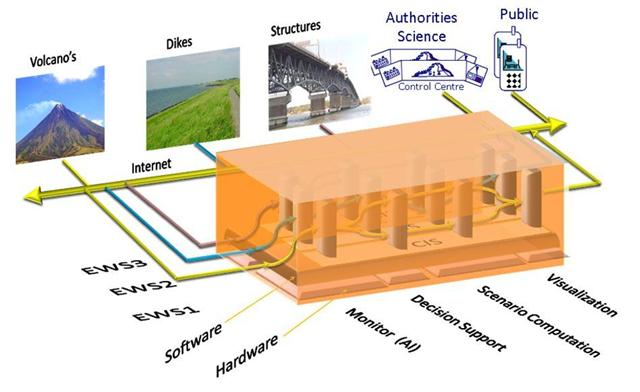
\includegraphics[scale=0.3]{concept.png}
\caption{Bron: \url{http://urbanflood.eu/aboutus.aspx}}
\end{figure}
\end{columns}
\end{frame}
\section{Doel Flood Simulation Browser}
\begin{frame}
\frametitle{Doel Flood Simulation Browser}
\begin{columns}[c]
\column{5cm}
\begin{itemize}
\item Visualisatie laten zien
\item Informeren over overstromingsgebied
\item Zien wat er als eerst onderwater gaat
\item Evacuatie routes
\item Hulpdienst routes
\item Browse door alle simulaties
\item Nieuwe simulatie uitvoeren
\end{itemize}
\column{5cm}
\begin{figure}
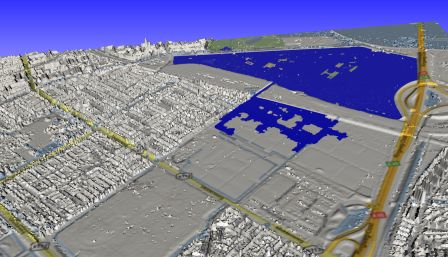
\includegraphics[scale=0.5]{simulation.png}
\caption{Bron: \url{http://urbanflood.eu/default.aspx}}
\end{figure}
\end{columns}
\end{frame}
\section{De requirements}
\begin{frame}
\frametitle{Requirements}
\begin{itemize}
\item Browser geschikt maken voor Tablets
\item Server levert plaatjes + coördinaten (Bounding Box)
\item Plaatjes over Google maps leggen - uitgebreid API support voor overlays
\item Intuïtief design
\item Taal/framework keuze
\item Mijn eis is: Crossplatform
\end{itemize}
\end{frame}
\section{App Design}
\begin{frame}
\frametitle{App Design}
\begin{columns}[c]
\column{5cm}
\begin{itemize}
\item Hoe mensen tablets vasthouden (Clark, 2012)
\item Letten op hierachie in importantie bij plaatsing componenten
\item Weergeven van simulaties (Locaties en bijbehorende simulaties)
\item Simulatiestappen kunnen doorlopen (controls).
\end{itemize}
\column{5cm}
\begin{figure}
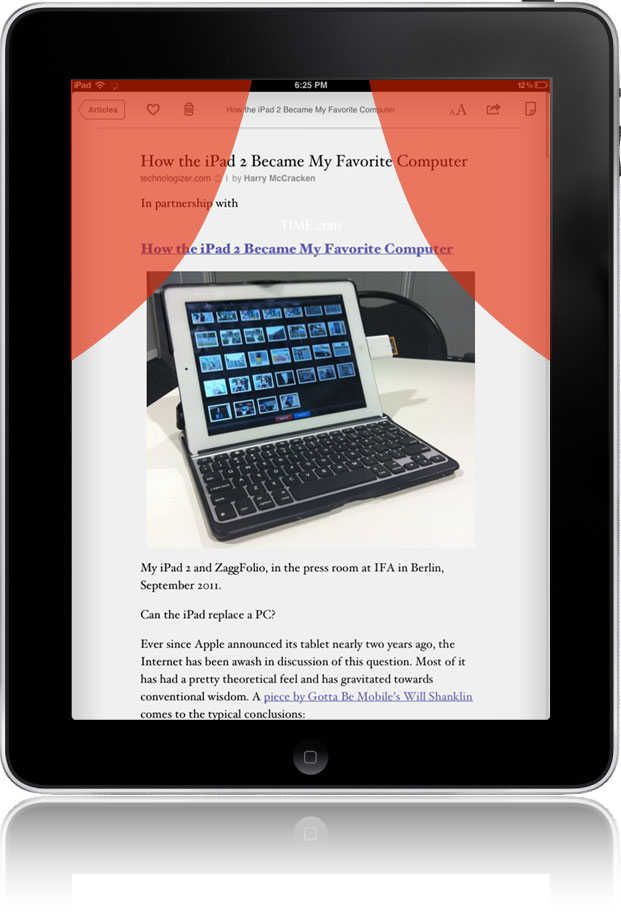
\includegraphics[scale=0.2]{touch.png}
\caption{Bron: \url{} (Clark 2012)}
\end{figure}
\end{columns}
\end{frame}
\section{Platform keuze}
\begin{frame}
\frametitle{Platform keuze}
\begin{itemize}
\item 
	\begin{itemize}
		\item iOS Objective C - niet crossplatform - hoge leercurve
			\item Android Java - idem
		\item jQuery Mobile -  problemen met fixed headers \& footers, combinatie PhoneGap
		\item Titanium - Makkelijk, maar vrij groot, veel geheugen gebruik. Design anders op andere telefoons en niet ECHT crossplatform
	\end{itemize}
\item Sencha Touch 2
\item Voordelen
		\begin{itemize}
		\item Crossplatform
		\item MVC Design Pattern
		\item Mobiele website of App
		\item Android en iOS
		\item Geen PhoneGap nodig
		\end{itemize}
\item Nadelen vooraf
		\begin{itemize}
				\item Verschilt veel met huidige persoonlijke kennis webtechnologiën
				\item Highlevel specificatie
				\item Mogelijk onvoorziene problemen
		\end{itemize}
\end{itemize}
\end{frame}
\section{Implementatie}
\begin{frame}
\frametitle{Implementatie}
\begin{columns}
\column{5cm}
\begin{itemize}
\item Sencha Touch 2
\item Layout
\item Flex 1, 2
\item List Objecten
\item Map Object
\end{itemize}
\column{5cm}
\begin{figure}
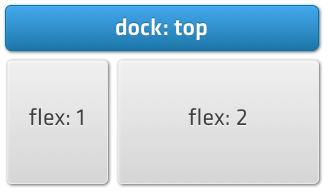
\includegraphics[scale=0.3]{docktop.png}
\end{figure}
\begin{figure}
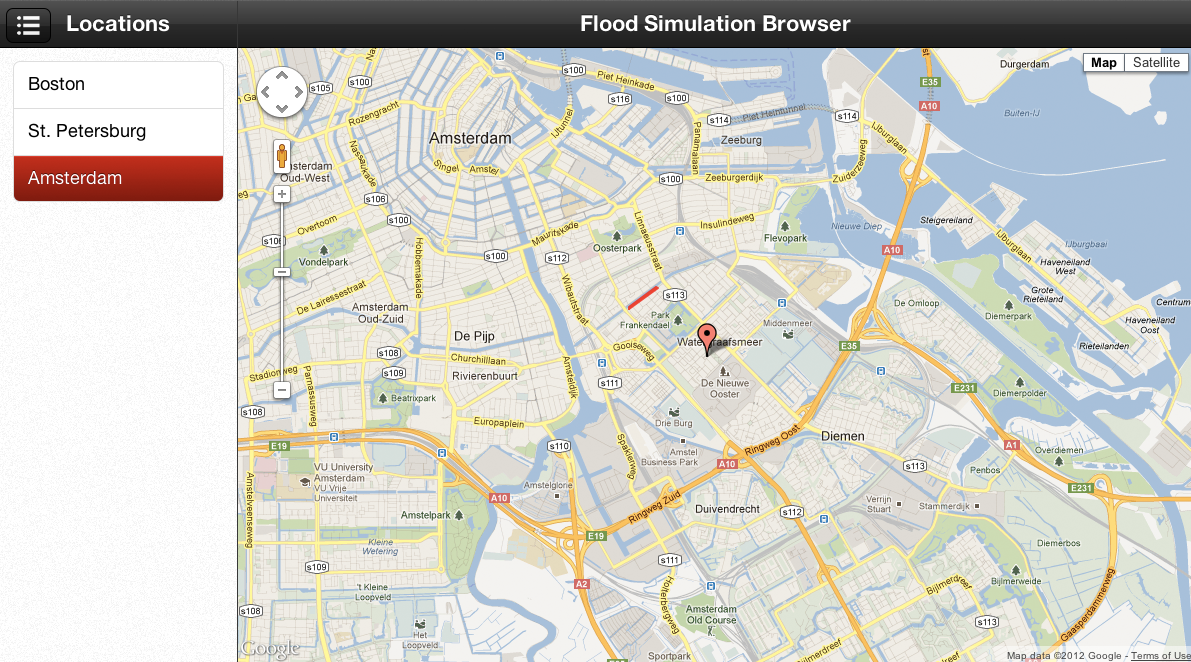
\includegraphics[scale=0.1]{ui/fsb_layout.png}
\end{figure}
\end{columns}
\end{frame}
\begin{frame}
\begin{itemize}
\item List \& Stores
\end{itemize}
\begin{figure}[h!]
\xymatrix{
  *+<5ex>[F]{Store}\ar[r]^{\txt<5pc>{fields}} &   *+<5ex>[F]{List}\ar[r] & 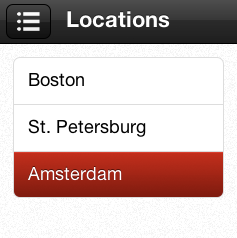
\includegraphics[scale=0.2]{ui/citieslist.png}\ar[dr] \\
  *+<5ex>[F]{Store}\ar[r]^{\txt<5pc>{fields}} &   *+<5ex>[F]{List}\ar[rr] & & 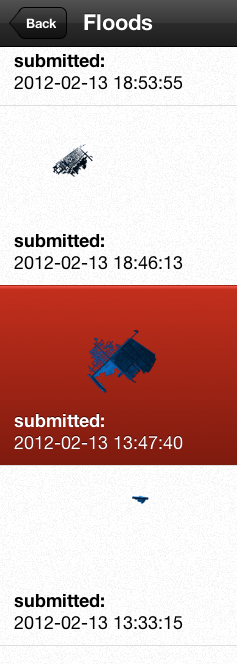
\includegraphics[scale=0.2]{ui/simselected.png}
}
\caption{Store and List}
\end{figure}
\end{frame}
\begin{frame}
\frametitle{Simulatie}
\begin{itemize}
\item Start simulatie
\item Controls, \\
        next step, prev step, play forward, play backwards
\item Tap \& Drag
\end{itemize}
\begin{figure}
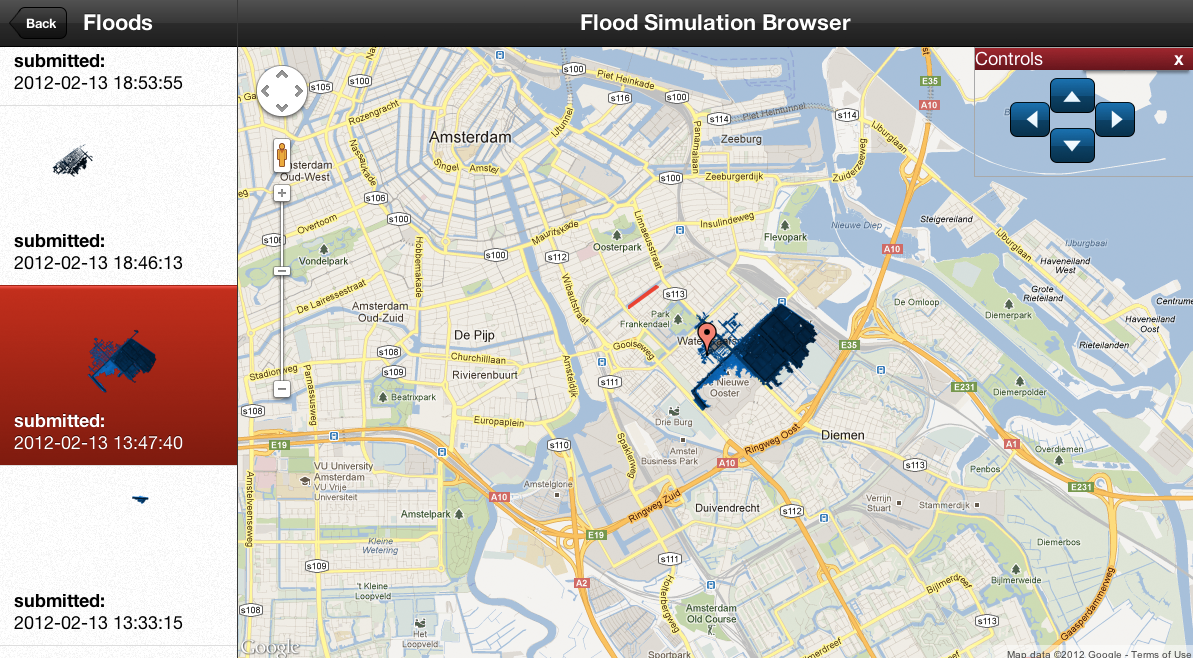
\includegraphics[scale=0.2]{ui/simselected_full.png}
\end{figure}
\end{frame}
\begin{frame}
\begin{itemize}
\frametitle{Volume Chart}
\item Tap op de kaart
\item Volume informatie van dichtsbijzijnde locatie van tap
\item Tap \& Drag
\end{itemize}
\begin{figure}
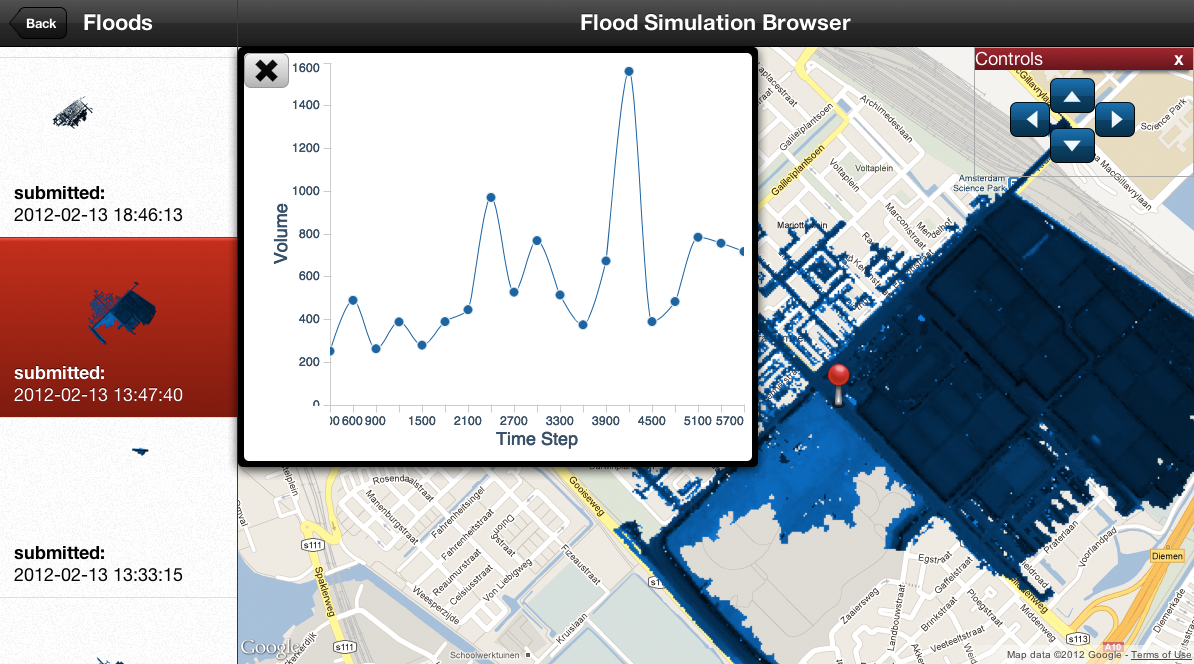
\includegraphics[scale=0.2]{ui/floodchart.png}
\end{figure}
\end{frame}
\begin{frame}
\begin{itemize}
\frametitle{Simulatie Mensen}
\item Selecteer simulatie Lsm
\item Tap locatie, tap simulatie
\end{itemize}
\begin{figure}
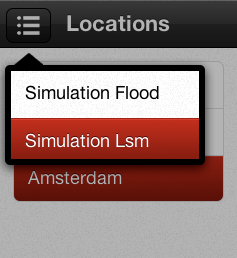
\includegraphics[scale=0.2]{ui/select_lsm.png}
\end{figure}
\begin{figure}
	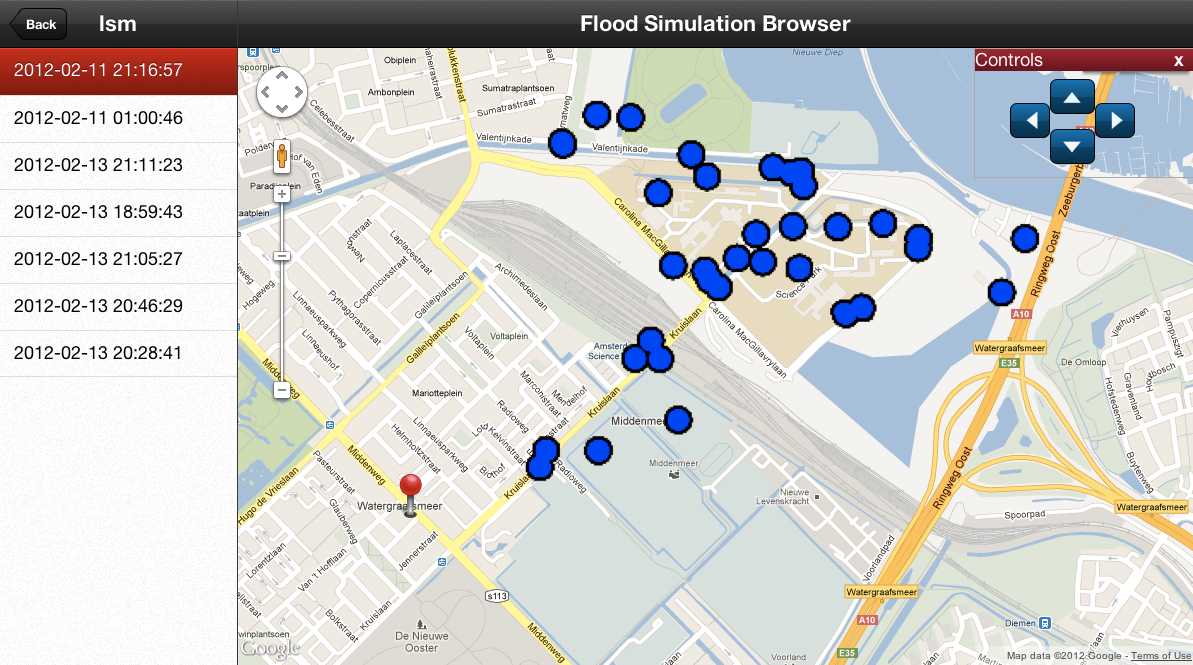
\includegraphics[scale=0.2]{ui/lsm.png}
	\caption{lsm}
\end{figure}
\end{frame}
\begin{frame}
\begin{itemize}
\frametitle{Deployment}
\item Test in Browser
\item Build: \textit{sencha app build native}
\begin{itemize}
	\item iOSSimulator
	\item iOS
	\item Android
	\item AndroidEmulator
\end{itemize}
\end{itemize}
\end{frame}

\section{Server Testing}
\begin{frame}[fragile]
\begin{itemize}
\item Tool: Siege
\item \url{sangkil.science.uva.nl}
\item file met verschillende requests, random uitgevoerd
\item Concurrente processen
\item Herhalingen
\end{itemize}
\begin{lstlisting}
#!/bin/bash
rep=(10 50 100 200 300 400 500)
for i in "${rep[@]}"
do
	siege -i -b -f /path/to/requests_file.txt -c $i -r $1
done
\end{lstlisting}
\end{frame}
\begin{frame}
\begin{figure}
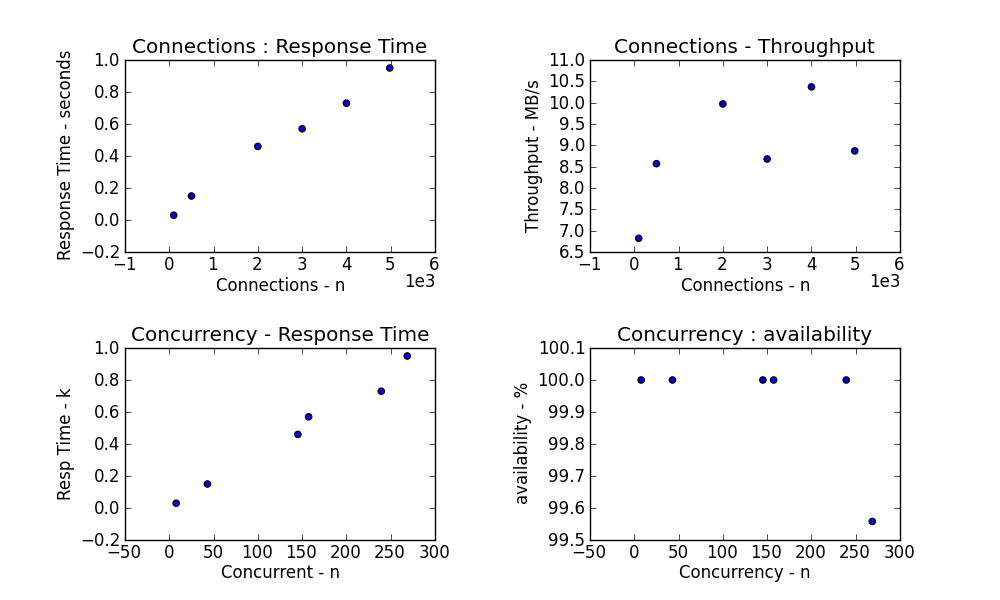
\includegraphics[scale=0.4]{siege_10r.png}
%siege_100r.log.png
%siege_200r.log.png}
\caption{10 repetities, getest: 10 50 200 300 400 500 concurrent}
\end{figure}
\end{frame}
\begin{frame}
\begin{figure}
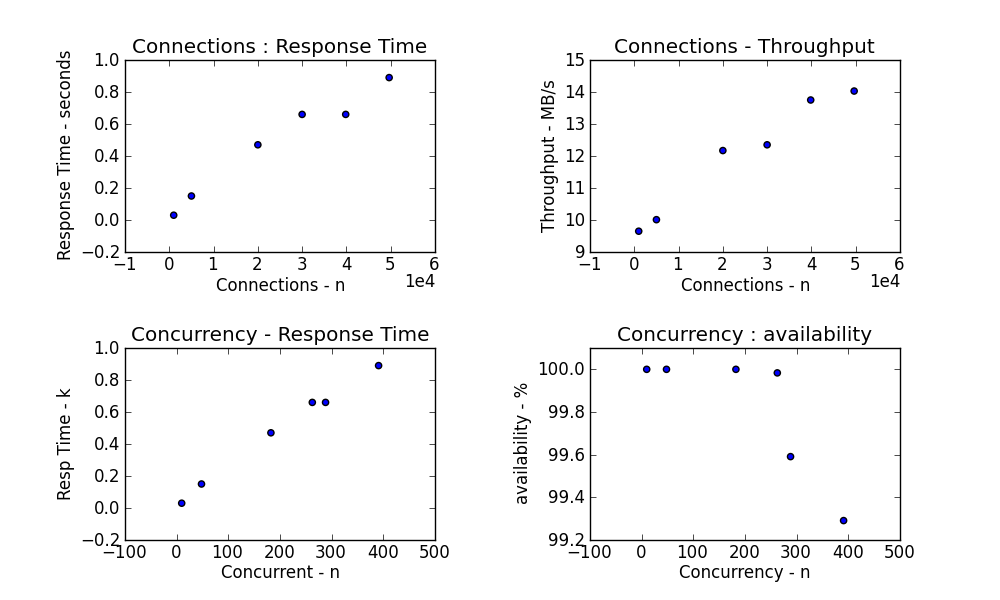
\includegraphics[scale=0.4]{siege_100r.png}
%siege_100r.log.png
%siege_200r.log.png}
\caption{100 repetities, test: 10 50 200 300 400 500 concurrent}
\end{figure}
\end{frame}

\begin{frame}
\begin{figure}
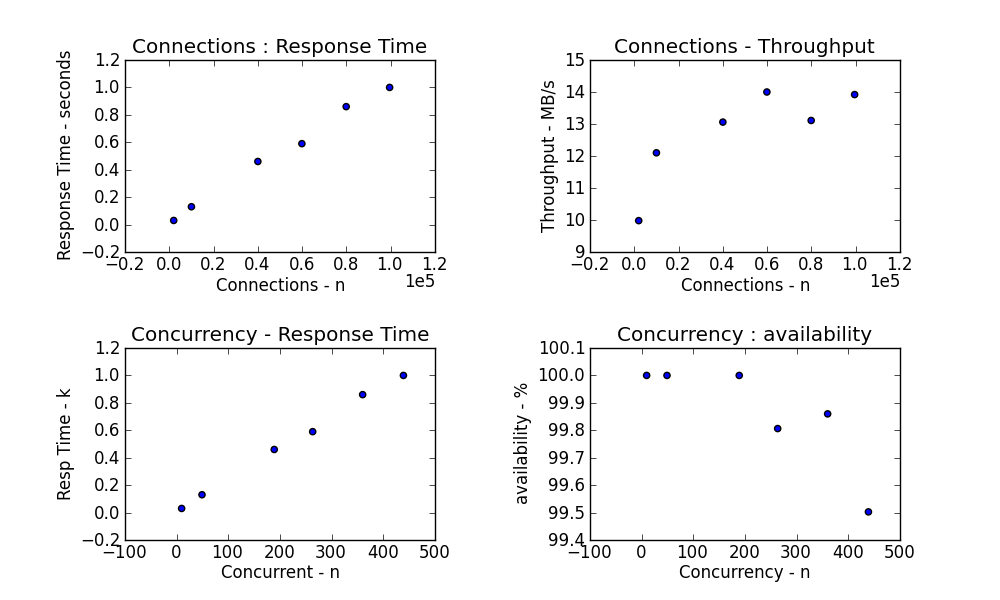
\includegraphics[scale=0.4]{siege_200r.png}
%siege_100r.log.png
%siege_200r.log.png}
\caption{200 repetities, getest: 10 50 200 300 400 500 concurrent}
\end{figure}
\end{frame}

\section{Referenties}
\begin{frame}
\begin{thebibliography}{9}
\frametitle{Referenties}
\bibitem{urban flood}
  Urban Flood Project,
  \url{http://urbanflood.eu/default.aspx}.
  Retrieved 9 april
\bibitem{Sencha Touch}
	Sencha Touch 2.
	\url{http://docs.sencha.com/touch/2-0/}.
	Retrieved 9 april
\bibitem{Google Maps API}
	Google Maps API,
	\url{https://developers.google.com/maps/}.
	Retrieved 9 april
\bibitem{PhoneGap}
	PhoneGap
	\url{http://www.PhoneGap.com}.
	Retrieved 9 april
\bibitem{Titanium Mobile}
	Titanium Appcelerator,
	\url{http://www.appcelerator.com/}.
	Retrieved 9 april
\end{thebibliography}
\end{frame}
\begin{frame}
\bibliographystyle{plain}
\bibliography{references}
\end{frame}
\end{document}